\documentclass[12pt]{article}
\usepackage{geometry}                % See geometry.pdf to learn the layout options. There are lots.
\geometry{letterpaper}                   % ... or a4paper or a5paper or ... 
%\geometry{landscape}                % Activate for for rotated page geometry
\usepackage[parfill]{parskip}    % Activate to begin paragraphs with an empty line rather than an indent
\usepackage{./styles/daves,fancyhdr,natbib,graphicx,dcolumn,amsmath,lastpage,url}
\usepackage{amsmath,amssymb,epstopdf,longtable}
\usepackage[final]{pdfpages}
\DeclareGraphicsRule{.tif}{png}{.png}{`convert #1 `dirname #1`/`basename #1 .tif`.png}
\pagestyle{fancy}
\lhead{CE 5362 -- Surface WaterModeling}
\rhead{SPRING 2020}
\lfoot{}
\cfoot{}
\rfoot{Page \thepage\ of \pageref{LastPage}}
\renewcommand\headrulewidth{0pt}



\begin{document}
\begin{center}
{\textbf{{ CE 5362 Surface Water Modeling} \\ {Project 8}}}
\end{center}

\section*{{Introduction and Purpose}}
SToRM is a component of the USGS Multi-Dimensional Surface Water Modeling System \citep{mdswms2012}
SToRM is one of a generation of recently available 2--D hydrodynamic models available without charge or for low cost. 
This project is to gain experience using the model to study the time-varying behavior of confluence of two streams 

\section*{{Problem Background}}
Figure \ref{fig:OrdinaryBasin} is a plan view map of a stream confluence, conceptualized in SToRM.  The inflows are the leftmost boundaries, and the outflow is the rightmost boundary.

%Figure \ref{fig:BasinInBasin}

\begin{figure}[h!] %  figure placement: here, top, bottom, or page
   \centering
   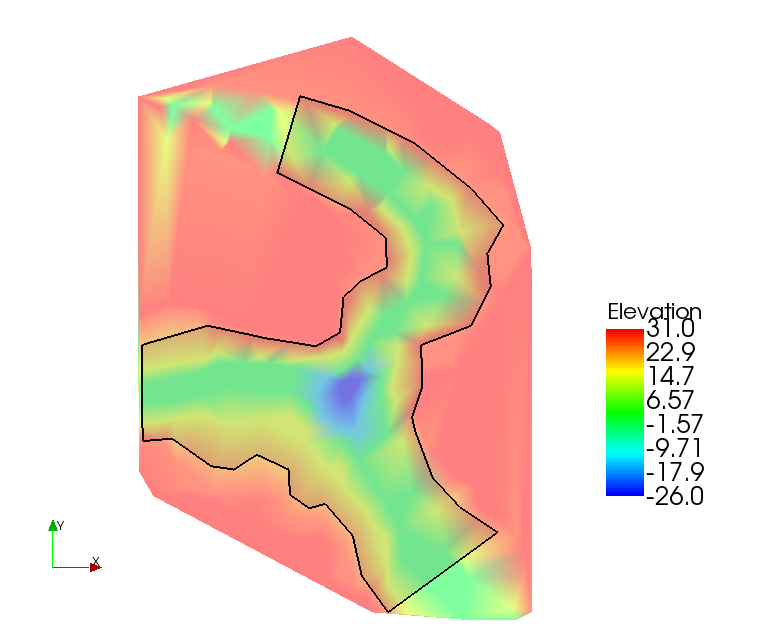
\includegraphics[height=3.5in]{OrdinaryBasin.png} 
   \caption{Aerial view of confluence with elevation scale shown. The portion outside area of interest is set to elevation 31 meters.}
   \label{fig:OrdinaryBasin}
\end{figure}

%\begin{figure}[h!] %  figure placement: here, top, bottom, or page
%   \centering
%   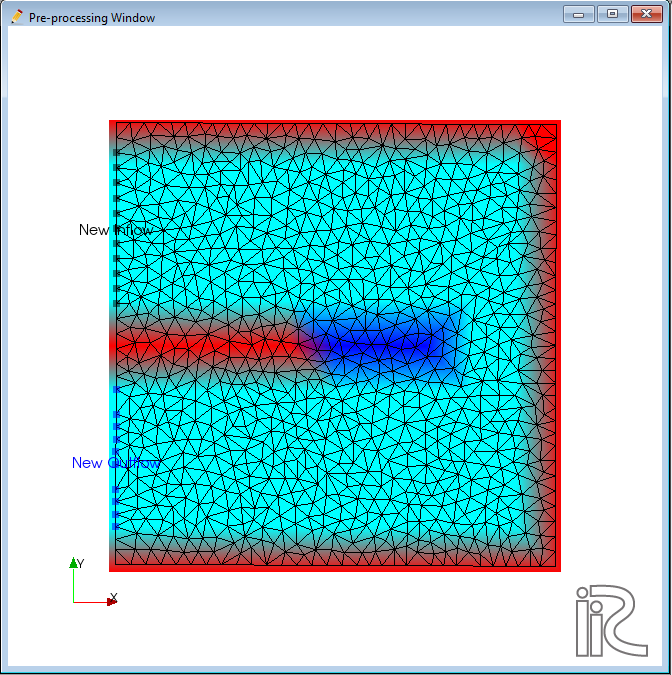
\includegraphics[height=3.5in]{BasinInBasin.png} 
%   \caption{Aerial view of Basin-In-Basin concept.   The red portion is elevation 4 meters, light blue is elevation 1 meters, and the dark blue is 0 meters. Inflow and outflow are shown.}
%   \label{fig:BasinInBasin}
%\end{figure}

The dark blue ``hole'' is thought to confer advantage by reducing velocity of water in its vicinity, thus suspended constituents could conceivably be captured in this region, if indeed the velocity field is affected.  

\subsubsection*{Topographic Model for the Confluence}
SToRM uses a topographic database in XYZ format.   Simple topographic files was built by digitizing a contour map of the study area using \texttt{G3DATA}, the file is named \url{bayou.jpg.txt.tpo}.

\subsubsection*{Boundary Conditions}
The inflow boundary conditions were obtained by digitizing hydrographs from Wang, et. al. 1996 using \texttt{G3DATA},
and are listed herein, first the inflow hydrographs, then a stage hydrograph for the downstream end.
\begin{verbatim}
buffalo bayou upstream
time(s)	q(cms)
874.0515933	12.64913151
9614.567527	12.64913151
20540.21244	28.46054591
33650.98634	69.57022333
42828.52807	120.1667494
52006.0698	177.0878412
56376.32777	284.6054591
59872.53414	382.6362283
64679.81791	480.6669975
70361.15326	572.373201
74731.41123	645.1057072
82160.84977	695.7022333
87842.18513	724.1627792
93960.54628	702.026799
104012.1396	660.9171216
110567.5266	622.969727
116248.8619	588.1846154
123241.2747	458.5310174
130233.6874	338.364268
138100.1517	243.4957816
146403.6419	151.7895782
159514.4158	104.355335
175684.3703	66.40794045
195350.5311	50.59652605
216327.7693	41.10967742
238616.085	31.62282878
266585.736	28.46054591
\end{verbatim}

\begin{verbatim}
whiteoak upstream
time(s)	q(cms)
0	6.324565757
12236.72231	25.29826303
26221.5478	60.08337469
37147.19272	148.6272953
41517.45068	202.3861042
48946.88923	265.6317618
56376.32777	471.1801489
60746.58574	800.0575682
63805.76631	1087.82531
65990.8953	1217.478908
67738.99848	1255.426303
69050.07587	1261.750868
72546.28225	1207.99206
80412.74659	961.333995
86531.10774	768.4347395
98330.80425	569.2109181
112752.6555	455.3687345
121930.1973	357.3379653
126300.4552	281.4431762
134166.9196	202.3861042
154270.1062	148.6272953
175684.3703	101.1930521
197972.6859	66.40794045
223320.1821	47.43424318
249978.7557	28.46054591
267022.7618	18.97369727
\end{verbatim}

\begin{verbatim}
buffalo bayou downstream
time(s)	stage(m)
0	0.855517268
3600	0.829221902
21600	0.847630963
43200	5.15802561
64800	6.236632103
66600	7.496430836
86400	2.774979436
108000	1.780747007
129600	1.394051388
151200	7.430356329
172800	4.580329805
194400	3.283308232
217800	2.437974098
241200	1.96207322
264600	1.628190963
286200	1.445657756
304200	1.346646963
324000	1.25942361
351000	1.164144829
378000	1.088578963
403200	1.049420732
432000	1.027644817
460800	0.997132927
496800	0.963971902
529200	0.939514927
558000	0.908042146
585000	0.905417988
603000	0.921159646
644400	0.913289805
684000	0.90279361
689400	0.898419159
\end{verbatim}

\section*{{Problem Statement}}
Build and run a SToRM model of the confluence, write a brief report (like a lab report) and include:
\begin{enumerate}
\item The velocity pattern in the confluence, at the peak White Oak discharge.
\item The velocity pattern in the confluence, at the peak Buffalo Bayou discharge.
\item The velocity pattern in the confluence, at the highest WSE in the confluence (as close as you can based on your output frequency).
\item Are the recirculation regions stable, or do they move about over the simulation time.
\end{enumerate}

\begin{thebibliography}{}

\bibitem[USGS, 2011]{storm2011}
{USGS Geomorphology Laboratory} (2011).
\newblock System for Transport and River Modeling.   
\url{http://wwwbrr.cr.usgs.gov/projects/GEOMORPH_Lab/project-SToRM.html} Webpage last accessed, 12 Jan 2012.

\bibitem[McDonald and others, 2012]{mdswms2012}
{McDonald, R.R., Nelson, J.M., and Bennett, J.P.}, (2012).  
\textsl{in press}. Multi-dimensional surface-water modeling system user's guide: U.S. Geological Survey Techniques and Methods, 6-B2, 136 p.

%\bibitem[Google Earth, 2011]{GoogleEarth2011}
%{Google Earth, Google Inc.}, (2011). 
%\url{http://www.google.com/earth/index.html} 
%1600 Amphitheatre Parkway Mountain View, CA, 94043
%%
%\bibitem[Golden Software, 2010]{surfer2010}
%{Golden Software, Inc.}, (2010). Surfer 10.
%809 14th Street, Golden, Colorado 80401-1866, U.S.A.
%Phone: 303-279-1021 Fax: 303-279-0909
%\url{www.GoldenSoftware.com}

%\bibitem[Dixon, J. 2011]{dixon2011}
%{Dixon, J.}, (2011). 
%A Relation Between Select Hydraulic Properties and Sediment
%Transport Volume Through Experimental Culvert Configurations
%and Techniques for Measuring Sediment Transport Volumes.
%MS Thesis, Department of Civil and Environmental Engineering, Texas Tech University, 117 p.

\end{thebibliography}

\end{document}